\subsection{收缩与截面}

命题8. 设 \(f\) 是从A到B的一个映射。如果存在一个映射 \(r\) （分别） \(s\) ) 从B到A，使得 \(r \circ f\) （分别） \(f \circ s\) 是 A（相应地，B）的恒等映射，则 \(f\) 是单射（相应地，满射）。反之，如果 \(f\) 是满射，则存在一个映射 \(s\) 将 B 映入 A，使得 \(f \circ s\) 是 B 的恒等映射。如果 \(f\) 是单射且如果 \(A \neq \emptyset\) ，则存在一个映射 \(r\) 将 B 映入 A，使得 \(r \circ f\) 是 A 的恒等映射。

如果存在从 \(B\) 到 \(A\) 的映射 \(r\) ，使得 \(r \circ f\) 是 \(A\) 上的恒等映射，那么等式 \(f(x) = f(y)\) （其中 \(x \in A\) 且 \(y \in A\) ）蕴含 \(x = r(f(x)) = r(f(y)) = y\) ，所以 \(f\) 是单射。如果存在从 \(B\) 到 \(A\) 的映射 \(s\) ，使得 \(f \circ s\) 是 \(B\) 上的恒等映射，则 \(B = f(s(B)) \subset f(A) \subset B\) ，故 \(f\) 是满射。如果 \(f\) 是满射，令 \(T\) 表示项 \(\tau_y(y \in A \text{ 且 } f(y) = x)\) 。我们有 \(f(T) = x\) （对于 \(x \in B\) ）；若 \(s\) 表示映射 \(x \to T (x \in B, T \in A)\) ，则 \(f \circ s\) 是 \(B\) 上的恒等映射。最后，假设 \(f\) 是单射且 \(A \neq \emptyset\) ，并设 \(a\) 为 \(A\) 的一个元素。关系

\[
" (y \in A \text {   且   } x = f (y)) \text {   或   } (y = a \text {   且   } x \in B - f (A))"
\]

蕴含 \((x, y) \in \mathbf{B} \times \mathbf{A}\) ，因而有一个图 \(\mathbf{R}\) （关于字母 \(x, y\) ）。由关于 \(f\) 的假设，此图是函数图，且以 \(\mathbf{B}\) 为定义域；我们就有 \(\mathbf{R}(x) = a\) （当 \(x \in \mathbf{B} - f(\mathbf{A})\) 时），且 \(f(\mathbf{R}(x)) = x\) （当 \(x \in f(\mathbf{A})\) 时）。因此，函数 \(r = (\mathbf{R}, \mathbf{B}, \mathbf{A})\) 满足： \(r \circ f\) 是 \(\mathbf{A}\) 上的恒等映射。

推论。设 A、B 为集合，设 f 为从 A 到 B 的映射，设 g 为从 B 到 A 的映射。如果 \(g \circ f\) 是 A 的恒等映射，并且如果 \(f \circ g\) 是 B 的恒等映射，则 f 和 g 是双射的，并且 \(g = \overline{f}^{1}\) .

定义 11。设 \(f\) 为 A 到 B 的单射（相应地，满射）。任意从 B 到 A 的映射 \(r\) （相应地，s），若 \(r \circ f\) （相应地， \(f \circ s\) ）是 A（相应地，B）上的恒等映射，则称为 \(f\) 的收缩（相应地，截面）。

的收缩（相应地，截面）。有时也使用左逆（相应地，右逆）这一术语来代替收缩（相应地，截面）。

如果 \(f\) 是单射（相应地，满射），且如果 \(r\) （分别） \(s\) ) 是 \(f\) ，那么 \(f\) 是 \(r\) （分别） \(s\) ）。因此，收缩映射是满射，截面映射是单射。

如果 \(f\) 是满射，且如果 \(s, s'\) 是 \(f\) 使得 \(s(\mathbf{B}) = s'(\mathbf{B})\) ，那么 \(s = s'\) ；因为如果 \(x \in \mathbf{B}\) , 存在 \(y \in \mathbf{B}\) 使得 \(s(x) = s'(y)\) ，并且我们有 \(x = f(s(x)) = f(s'(y)) = y\) ，因此 \(s(x) = s'(x)\) ，从而 \(s = s'\) 因此，一个截面 \(s\) 由该集合唯一确定 \(s(\mathbf{B})\) 。滥用语言时，集合 \(s(\mathbf{B})\) 有时被称为 \(f\) .

定理1. 设 \(f\) 为从A到B的映射，设 \(f'\) 为从B到C的映射，且设 \(f'' = f' \circ f\) 。则：

\begin{enumerate}
\def\labelenumi{(\alph{enumi})}
\item
  如果 \(f\) 并且 \(f'\) 都是单射，则 \(f''\) 是一个单射。如果 \(r, r'\) 分别是 \(f, f'\) 的收缩，那么 \(r \circ r'\) 是 \(f''\) .
\item
  如果 \(f\) 并且 \(f'\) 都是满射，则 \(f''\) 是一个满射。如果 \(s, s'\) 是 \(f, f'\) 的收缩，那么 \(s \circ s'\) 是 \(f''\) .
\item
  如果 \(f''\) 若为单射，则 \(f\) 是一个单射。如果 \(r''\) 是 \(f''\) ，那么 \(r'' \circ f'\) 是 \(f\) .
\item
  如果 \(f''\) 是一个满射，则 \(f'\) 是一个满射。如果 \(s''\) 是 \(f''\) ，那么 \(f \circ s''\) 是 \(f'\) .
\item
  如果 \(f''\) 是一个满射且 \(f'\) 的一个截面，则 \(f\) 是一个满射。如果 \(s''\) 是 \(f''\) ，那么 \(s'' \circ f'\) 是 \(f\) .
\item
  如果 \(f''\) 是一个单射，且 \(f\) 一个满射，则 \(f'\) 是一个单射。如果 \(r''\) 是 \(f''\) ，那么 \(f \circ r''\) 是 \(f'\) .
\end{enumerate}

对于每一个集合E，令 \(I_{E}\) 表示 E 的恒等映射。

\begin{enumerate}
\def\labelenumi{(\alph{enumi})}
\tightlist
\item
  我们有 \(r \circ f = I_A\) 并且 \(r' \circ f' = I_B\) ，因此
\end{enumerate}

\[
\left(r \circ r ^ {\prime}\right) \circ \left(f ^ {\prime} \circ f\right) = r \circ I _ {B} \circ f = r \circ f = I _ {A}.
\]

如果 \(f\) 并且 \(f'\) 都是单射，则 \(f''\) 是单射，根据命题8，如果 \(A \neq \emptyset\) ，且平凡地，如果 \(A = \emptyset\) .

\begin{enumerate}
\def\labelenumi{(\alph{enumi})}
\setcounter{enumi}{1}
\tightlist
\item
  我们有 \(f \circ s = \mathbf{I}_{\mathrm{B}}\) 并且 \(f' \circ s' = \mathbf{I}_{\mathrm{C}}\) ，因此
\end{enumerate}

\[
(f ^ {\prime} \circ f) (s \circ s ^ {\prime}) = f ^ {\prime} \circ I _ {B} \circ s ^ {\prime} = f ^ {\prime} \circ s ^ {\prime} = I _ {C}.
\]

如果 \(f\) 并且 \(f'\) 是满射， \(f''\) 于是根据命题8，这是一个满射。

\begin{enumerate}
\def\labelenumi{(\alph{enumi})}
\setcounter{enumi}{2}
\item
  我们有 \(r'' \circ f'' = I_A\) ，因此 \((r'' \circ f') \circ f = r'' \circ f'' = I_A\) 。如果 \(f''\) 若为单射，则 \(f\) 是单射，根据命题8，如果 \(A \neq \emptyset\) ，且平凡地，如果 \(A = \emptyset\) .
\item
  我们有 \(f'' \circ s'' = I_C\) ，因此 \(f' \circ (f \circ s'') = f'' \circ s'' = I_C\) 。如果 \(f''\) 是一个满射，则 \(f'\) 是满射，依据命题8。
\item
  我们有 \(f'' \circ s'' = I_G\) ，以及 \(f'\) 由(d)可知是一个双射。因此
\end{enumerate}

\[
\begin{array}{r l} f \circ (s ^ {\prime \prime} \circ f ^ {\prime}) = (\bar {f} ^ {1 ^ {\prime}} \circ f ^ {\prime}) \circ f \circ (s ^ {\prime \prime} \circ f ^ {\prime}) & = \bar {f} ^ {1 ^ {\prime}} \circ (f ^ {\prime \prime} \circ s ^ {\prime \prime}) \circ f ^ {\prime} \\ & = \bar {f} ^ {1 ^ {\prime}} \circ I _ {C} \circ f ^ {\prime} = \bar {f} ^ {1 ^ {\prime}} \circ f ^ {\prime} = I _ {B}. \end{array}
\]

如果 \(f''\) 是一个满射且 \(f'\) 一个单射， \(f\) 于是根据命题8，这是一个满射。

\begin{enumerate}
\def\labelenumi{(\alph{enumi})}
\setcounter{enumi}{5}
\tightlist
\item
  我们有 \(r'' \circ f'' = I_A\) ，以及 \(f\) 由(c)可知是一个双射。因此
\end{enumerate}

\[
\begin{array}{r l} \left(f \circ r ^ {\prime \prime}\right) \circ f ^ {\prime} = \left(f \circ r ^ {\prime \prime}\right) \circ f ^ {\prime} \circ \left(f \circ \overline {{f}} ^ {1}\right) & = f \circ \left(r ^ {\prime \prime} \circ f ^ {\prime \prime}\right) \circ \overline {{f}} ^ {1} = f \circ I _ {A} \circ \overline {{f}} ^ {1} \\ & = f \circ \overline {{f}} ^ {1} = I _ {B}. \end{array}
\]

如果 \(f''\) 是一个单射，且 \(f\) 一个满射，则 \(f'\) 是单射，根据命题8，如果 \(A \neq \emptyset\) ，且平凡地，如果 \(A = \emptyset\) （因为此时我们有 \(B = f\langle A\rangle = \emptyset\) ).

命题9。(a) 设E、F、G为集合，设g为E到F上的映射，f为E到G内的映射。则存在F到G内的映射h，使得 \(f = h \circ g\) 当且仅当关系 \(g(x) = g(y)\) （其中 \(x \in E\) , \(y \in E\) )蕴含关系 \(f(x) = f(y)\) 。此时映射h由f唯一确定；若s是g的一个截面，则有 \(h = f \circ s\) .

\pandocbounded{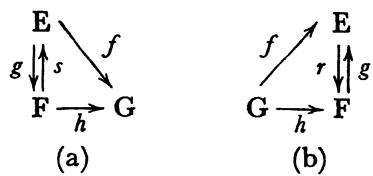
\includegraphics[keepaspectratio]{images/part001_ef8e01c05a3dcb28772fb1963be4c012627d42ff76089463ce60c193ac31650a.jpg}}

\begin{enumerate}
\def\labelenumi{(\alph{enumi})}
\setcounter{enumi}{1}
\item
  设E、F、G为集合，设g为F到E的一个单射，并设f为G到E的一个映射。则存在G到F的一个映射h，使得 \(f = g \circ h\) 当且仅当 \(f(\mathbf{G}) \subset f(\mathbf{F})\) 映射 h 由 f 唯一确定；若 r 是 g 的一个收缩，则我们有 \(h = r \circ f\) .
\item
  如果 \(f = h \circ g\) ，关系 \(g(x) = g(y)\) （其中 \(x \in \mathbf{E}\) , \(y \in \mathbf{E}\) ) 显然蕴含 \(f(x) = f(y)\) 。并且对于每个截面 \(s\) 的 \(g\) 我们拥有
\end{enumerate}

\[
h = h \circ (g \circ s) = f \circ s,
\]

，这表明 h 由 f 唯一确定。反之，假设关系 \(g(x) = g(y)\) 蕴含 \(f(x) = f(y)\) ；设 s 是 \(g\) 的一个截面，并令 \(h = f \circ s\) ；则对每个 \(x \in \mathbf{E}\) 都有 \(g(s(g(x))) = g(x)\) ，因而 \(f(s(g(x))) = f(x)\) ，即 \(h(g(x)) = f(x)\) 。因此 \(f = h \circ g\) .

\begin{enumerate}
\def\labelenumi{(\alph{enumi})}
\setcounter{enumi}{1}
\tightlist
\item
  如果 \(f = g \circ h\) ，那么显然 \(f(\mathbf{G}) \subset f(\mathbf{F})\) ，并且对于每个收缩 \(r\) 的 \(g\) 我们拥有 \(h = (r \circ g) \circ h = r \circ f\) ，这表明 \(h\) 由...唯一确定 \(f\) 相反，假设 \(f(\mathbf{G}) \subset f(\mathbf{F})\) ；令 \(r\) 为 \(g\) ，并放置 \(h = r \circ f\) ；对于每一个 \(x \in \mathbf{G}\) , 存在 \(y \in \mathbf{F}\) 使得 \(f(x) = g(y)\) ，因此
\end{enumerate}

\[
g (h (x)) = g (r (f (x))) = g (r (g (y))) = g (y) = f (x)
\]

因此 \(f = g \circ h\) .

